\documentclass[1p]{elsarticle_modified}
%\bibliographystyle{elsarticle-num}

%\usepackage[colorlinks]{hyperref}
%\usepackage{abbrmath_seonhwa} %\Abb, \Ascr, \Acal ,\Abf, \Afrak
\usepackage{amsfonts}
\usepackage{amssymb}
\usepackage{amsmath}
\usepackage{amsthm}
\usepackage{scalefnt}
\usepackage{amsbsy}
\usepackage{kotex}
\usepackage{caption}
\usepackage{subfig}
\usepackage{color}
\usepackage{graphicx}
\usepackage{xcolor} %% white, black, red, green, blue, cyan, magenta, yellow
\usepackage{float}
\usepackage{setspace}
\usepackage{hyperref}

\usepackage{tikz}
\usetikzlibrary{arrows}

\usepackage{multirow}
\usepackage{array} % fixed length table
\usepackage{hhline}

%%%%%%%%%%%%%%%%%%%%%
\makeatletter
\renewcommand*\env@matrix[1][\arraystretch]{%
	\edef\arraystretch{#1}%
	\hskip -\arraycolsep
	\let\@ifnextchar\new@ifnextchar
	\array{*\c@MaxMatrixCols c}}
\makeatother %https://tex.stackexchange.com/questions/14071/how-can-i-increase-the-line-spacing-in-a-matrix
%%%%%%%%%%%%%%%

\usepackage[normalem]{ulem}

\newcommand{\msout}[1]{\ifmmode\text{\sout{\ensuremath{#1}}}\else\sout{#1}\fi}
%SOURCE: \msout is \stkout macro in https://tex.stackexchange.com/questions/20609/strikeout-in-math-mode

\newcommand{\cancel}[1]{
	\ifmmode
	{\color{red}\msout{#1}}
	\else
	{\color{red}\sout{#1}}
	\fi
}

\newcommand{\add}[1]{
	{\color{blue}\uwave{#1}}
}

\newcommand{\replace}[2]{
	\ifmmode
	{\color{red}\msout{#1}}{\color{blue}\uwave{#2}}
	\else
	{\color{red}\sout{#1}}{\color{blue}\uwave{#2}}
	\fi
}

\newcommand{\Sol}{\mathcal{S}} %segment
\newcommand{\D}{D} %diagram
\newcommand{\A}{\mathcal{A}} %arc


%%%%%%%%%%%%%%%%%%%%%%%%%%%%%5 test

\def\sl{\operatorname{\textup{SL}}(2,\Cbb)}
\def\psl{\operatorname{\textup{PSL}}(2,\Cbb)}
\def\quan{\mkern 1mu \triangleright \mkern 1mu}

\theoremstyle{definition}
\newtheorem{thm}{Theorem}[section]
\newtheorem{prop}[thm]{Proposition}
\newtheorem{lem}[thm]{Lemma}
\newtheorem{ques}[thm]{Question}
\newtheorem{cor}[thm]{Corollary}
\newtheorem{defn}[thm]{Definition}
\newtheorem{exam}[thm]{Example}
\newtheorem{rmk}[thm]{Remark}
\newtheorem{alg}[thm]{Algorithm}

\newcommand{\I}{\sqrt{-1}}
\begin{document}

%\begin{frontmatter}
%
%\title{Boundary parabolic representations of knots up to 8 crossings}
%
%%% Group authors per affiliation:
%\author{Yunhi Cho} 
%\address{Department of Mathematics, University of Seoul, Seoul, Korea}
%\ead{yhcho@uos.ac.kr}
%
%
%\author{Seonhwa Kim} %\fnref{s_kim}}
%\address{Center for Geometry and Physics, Institute for Basic Science, Pohang, 37673, Korea}
%\ead{ryeona17@ibs.re.kr}
%
%\author{Hyuk Kim}
%\address{Department of Mathematical Sciences, Seoul National University, Seoul 08826, Korea}
%\ead{hyukkim@snu.ac.kr}
%
%\author{Seokbeom Yoon}
%\address{Department of Mathematical Sciences, Seoul National University, Seoul, 08826,  Korea}
%\ead{sbyoon15@snu.ac.kr}
%
%\begin{abstract}
%We find all boundary parabolic representation of knots up to 8 crossings.
%
%\end{abstract}
%\begin{keyword}
%    \MSC[2010] 57M25 
%\end{keyword}
%
%\end{frontmatter}

%\linenumbers
%\tableofcontents
%
\newcommand\colored[1]{\textcolor{white}{\rule[-0.35ex]{0.8em}{1.4ex}}\kern-0.8em\color{red} #1}%
%\newcommand\colored[1]{\textcolor{white}{ #1}\kern-2.17ex	\textcolor{white}{ #1}\kern-1.81ex	\textcolor{white}{ #1}\kern-2.15ex\color{red}#1	}

{\Large $\underline{12a_{1125}~(K12a_{1125})}$}

\setlength{\tabcolsep}{10pt}
\renewcommand{\arraystretch}{1.6}
\vspace{1cm}\begin{tabular}{m{100pt}>{\centering\arraybackslash}m{274pt}}
\multirow{5}{120pt}{
	\centering
	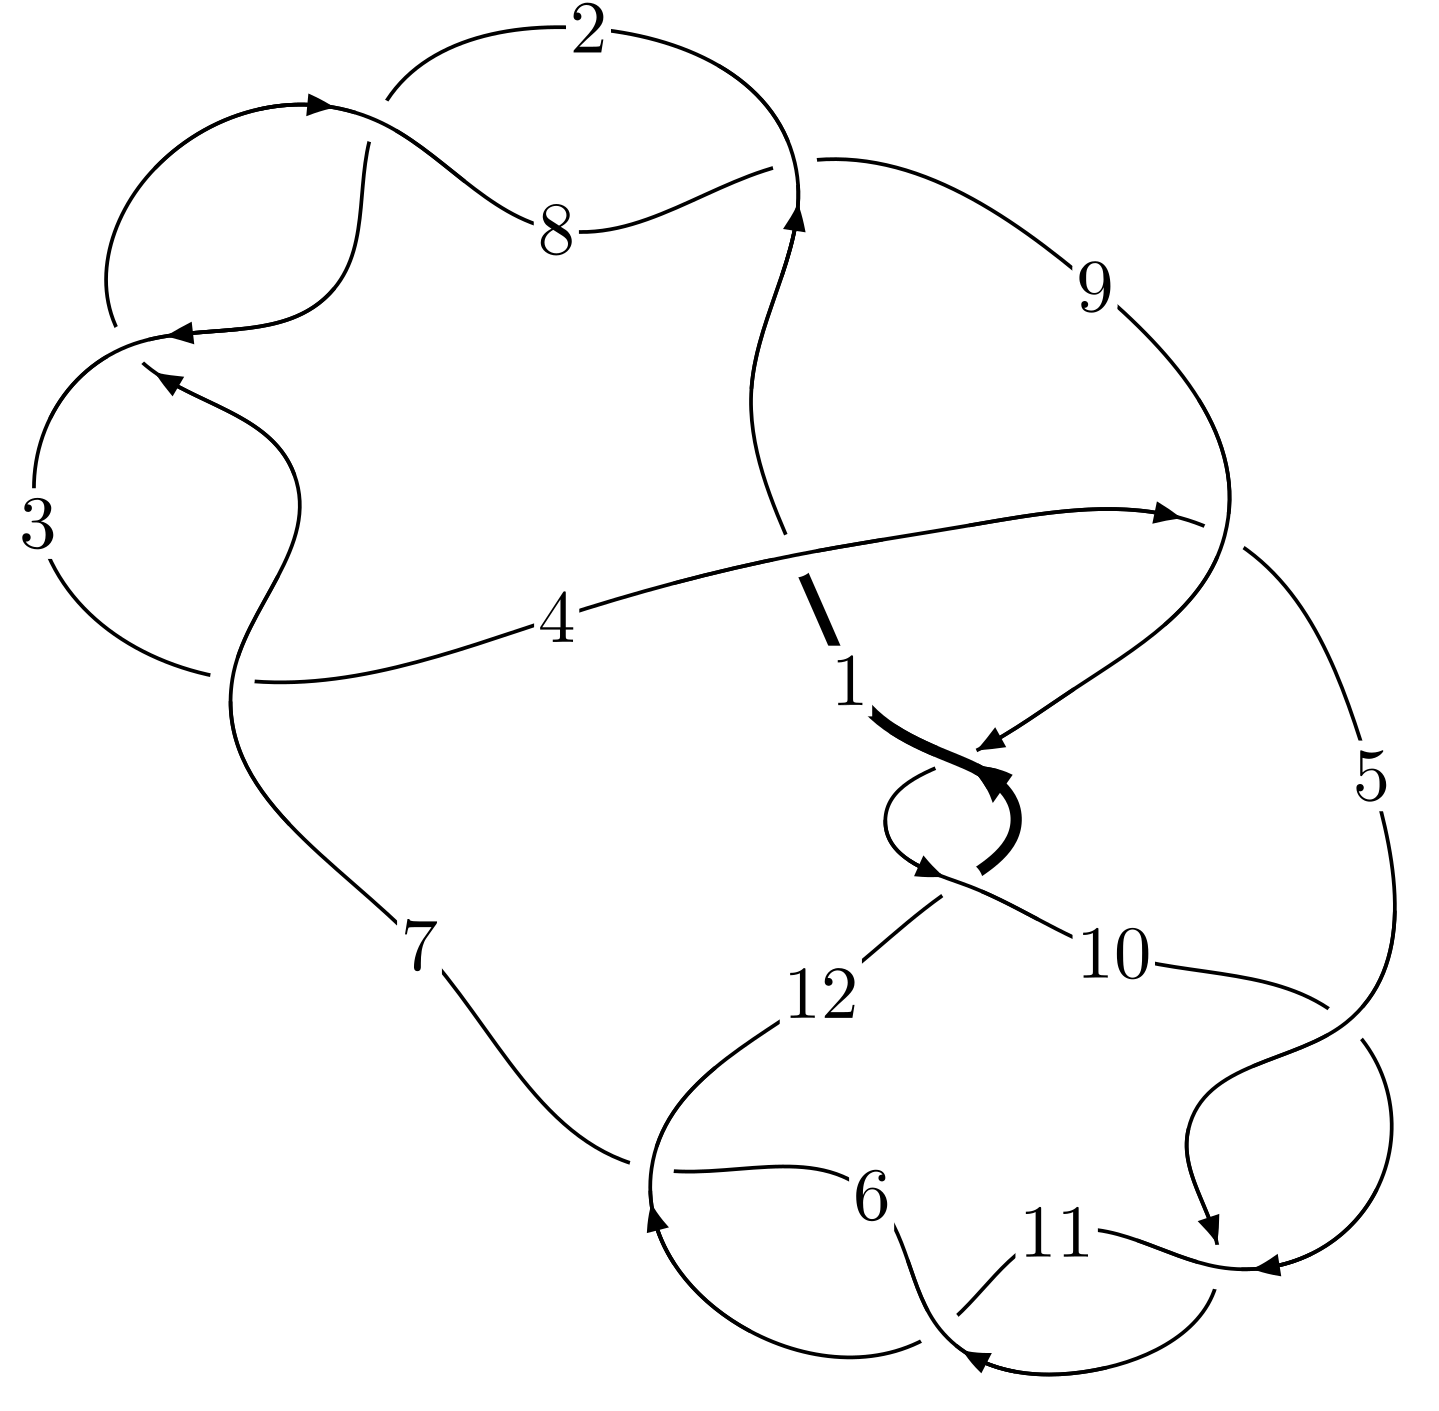
\includegraphics[width=112pt]{../../../GIT/diagram.site/Diagrams/png/1926_12a_1125.png}\\
\ \ \ A knot diagram\footnotemark}&
\allowdisplaybreaks
\textbf{Linearized knot diagam} \\
\cline{2-2}
 &
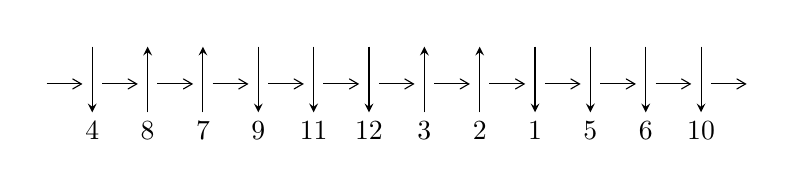
\begin{tikzpicture}[x=20pt, y=17pt]
	% nodes
	\node (C0) at (0, 0) {};
	\node (C1) at (1, 0) {};
	\node (C1U) at (1, +1) {};
	\node (C1D) at (1, -1) {4};

	\node (C2) at (2, 0) {};
	\node (C2U) at (2, +1) {};
	\node (C2D) at (2, -1) {8};

	\node (C3) at (3, 0) {};
	\node (C3U) at (3, +1) {};
	\node (C3D) at (3, -1) {7};

	\node (C4) at (4, 0) {};
	\node (C4U) at (4, +1) {};
	\node (C4D) at (4, -1) {9};

	\node (C5) at (5, 0) {};
	\node (C5U) at (5, +1) {};
	\node (C5D) at (5, -1) {11};

	\node (C6) at (6, 0) {};
	\node (C6U) at (6, +1) {};
	\node (C6D) at (6, -1) {12};

	\node (C7) at (7, 0) {};
	\node (C7U) at (7, +1) {};
	\node (C7D) at (7, -1) {3};

	\node (C8) at (8, 0) {};
	\node (C8U) at (8, +1) {};
	\node (C8D) at (8, -1) {2};

	\node (C9) at (9, 0) {};
	\node (C9U) at (9, +1) {};
	\node (C9D) at (9, -1) {1};

	\node (C10) at (10, 0) {};
	\node (C10U) at (10, +1) {};
	\node (C10D) at (10, -1) {5};

	\node (C11) at (11, 0) {};
	\node (C11U) at (11, +1) {};
	\node (C11D) at (11, -1) {6};

	\node (C12) at (12, 0) {};
	\node (C12U) at (12, +1) {};
	\node (C12D) at (12, -1) {10};
	\node (C13) at (13, 0) {};

	% arrows
	\draw[->,>={angle 60}]
	(C0) edge (C1) (C1) edge (C2) (C2) edge (C3) (C3) edge (C4) (C4) edge (C5) (C5) edge (C6) (C6) edge (C7) (C7) edge (C8) (C8) edge (C9) (C9) edge (C10) (C10) edge (C11) (C11) edge (C12) (C12) edge (C13) ;	\draw[->,>=stealth]
	(C1U) edge (C1D) (C2D) edge (C2U) (C3D) edge (C3U) (C4U) edge (C4D) (C5U) edge (C5D) (C6U) edge (C6D) (C7D) edge (C7U) (C8D) edge (C8U) (C9U) edge (C9D) (C10U) edge (C10D) (C11U) edge (C11D) (C12U) edge (C12D) ;
	\end{tikzpicture} \\
\hhline{~~} \\& 
\textbf{Solving Sequence} \\ \cline{2-2} 
 &
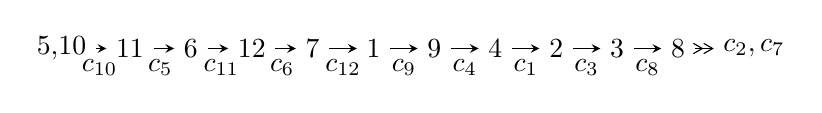
\begin{tikzpicture}[x=22pt, y=7pt]
	% node
	\node (A0) at (-1/8, 0) {5,10};
	\node (A1) at (1, 0) {11};
	\node (A2) at (2, 0) {6};
	\node (A3) at (3, 0) {12};
	\node (A4) at (4, 0) {7};
	\node (A5) at (5, 0) {1};
	\node (A6) at (6, 0) {9};
	\node (A7) at (7, 0) {4};
	\node (A8) at (8, 0) {2};
	\node (A9) at (9, 0) {3};
	\node (A10) at (10, 0) {8};
	\node (C1) at (1/2, -1) {$c_{10}$};
	\node (C2) at (3/2, -1) {$c_{5}$};
	\node (C3) at (5/2, -1) {$c_{11}$};
	\node (C4) at (7/2, -1) {$c_{6}$};
	\node (C5) at (9/2, -1) {$c_{12}$};
	\node (C6) at (11/2, -1) {$c_{9}$};
	\node (C7) at (13/2, -1) {$c_{4}$};
	\node (C8) at (15/2, -1) {$c_{1}$};
	\node (C9) at (17/2, -1) {$c_{3}$};
	\node (C10) at (19/2, -1) {$c_{8}$};
	\node (A11) at (45/4, 0) {$c_{2},c_{7}$};

	% edge
	\draw[->,>=stealth]	
	(A0) edge (A1) (A1) edge (A2) (A2) edge (A3) (A3) edge (A4) (A4) edge (A5) (A5) edge (A6) (A6) edge (A7) (A7) edge (A8) (A8) edge (A9) (A9) edge (A10) ;
	\draw[->>,>={angle 60}]	
	(A10) edge (A11);
\end{tikzpicture} \\ 

\end{tabular} \\

\footnotetext{
The image of knot diagram is generated by the software ``\textbf{Draw programme}" developed by Andrew Bartholomew(\url{http://www.layer8.co.uk/maths/draw/index.htm\#Running-draw}), where we modified some parts for our purpose(\url{https://github.com/CATsTAILs/LinksPainter}).
}\phantom \\ \newline 
\centering \textbf{Ideals for irreducible components\footnotemark of $X_{\text{par}}$} 
 
\begin{align*}
I^u_{1}&=\langle 
u^{50}+u^{49}+\cdots- u-1\rangle \\
\\
\end{align*}
\raggedright * 1 irreducible components of $\dim_{\mathbb{C}}=0$, with total 50 representations.\\
\footnotetext{All coefficients of polynomials are rational numbers. But the coefficients are sometimes approximated in decimal forms when there is not enough margin.}
\newpage
\renewcommand{\arraystretch}{1}
\centering \section*{I. $I^u_{1}= \langle u^{50}+u^{49}+\cdots- u-1 \rangle$}
\flushleft \textbf{(i) Arc colorings}\\
\begin{tabular}{m{7pt} m{180pt} m{7pt} m{180pt} }
\flushright $a_{5}=$&$\begin{pmatrix}0\\u\end{pmatrix}$ \\
\flushright $a_{10}=$&$\begin{pmatrix}1\\0\end{pmatrix}$ \\
\flushright $a_{11}=$&$\begin{pmatrix}1\\u^2\end{pmatrix}$ \\
\flushright $a_{6}=$&$\begin{pmatrix}- u\\- u^3+u\end{pmatrix}$ \\
\flushright $a_{12}=$&$\begin{pmatrix}- u^2+1\\- u^4+2 u^2\end{pmatrix}$ \\
\flushright $a_{7}=$&$\begin{pmatrix}u^3-2 u\\u^5-3 u^3+u\end{pmatrix}$ \\
\flushright $a_{1}=$&$\begin{pmatrix}u^4-3 u^2+1\\- u^4+2 u^2\end{pmatrix}$ \\
\flushright $a_{9}=$&$\begin{pmatrix}u^8-5 u^6+7 u^4-2 u^2+1\\- u^8+4 u^6-4 u^4\end{pmatrix}$ \\
\flushright $a_{4}=$&$\begin{pmatrix}u^{17}-10 u^{15}+39 u^{13}-74 u^{11}+71 u^9-38 u^7+18 u^5-4 u^3+u\\- u^{17}+9 u^{15}-31 u^{13}+50 u^{11}-37 u^9+12 u^7-4 u^5+u\end{pmatrix}$ \\
\flushright $a_{2}=$&$\begin{pmatrix}u^{30}-17 u^{28}+\cdots-2 u^2+1\\- u^{30}+16 u^{28}+\cdots-6 u^4+3 u^2\end{pmatrix}$ \\
\flushright $a_{3}=$&$\begin{pmatrix}u^{25}-14 u^{23}+\cdots-10 u^3+u\\u^{27}-15 u^{25}+\cdots+3 u^3+u\end{pmatrix}$ \\
\flushright $a_{8}=$&$\begin{pmatrix}u^{47}-26 u^{45}+\cdots+4 u^3-2 u\\u^{49}-27 u^{47}+\cdots+2 u^5+u\end{pmatrix}$\\&\end{tabular}
\flushleft \textbf{(ii) Obstruction class $= -1$}\\~\\
\flushleft \textbf{(iii) Cusp Shapes $= -4 u^{47}+104 u^{45}+\cdots-4 u-6$}\\~\\
\newpage\renewcommand{\arraystretch}{1}
\flushleft \textbf{(iv) u-Polynomials at the component}\newline \\
\begin{tabular}{m{50pt}|m{274pt}}
Crossings & \hspace{64pt}u-Polynomials at each crossing \\
\hline $$\begin{aligned}c_{1}\end{aligned}$$&$\begin{aligned}
&u^{50}-13 u^{49}+\cdots-53 u+3
\end{aligned}$\\
\hline $$\begin{aligned}c_{2},c_{3},c_{7}\\c_{8}\end{aligned}$$&$\begin{aligned}
&u^{50}- u^{49}+\cdots+u-1
\end{aligned}$\\
\hline $$\begin{aligned}c_{4}\end{aligned}$$&$\begin{aligned}
&u^{50}- u^{49}+\cdots+35 u-29
\end{aligned}$\\
\hline $$\begin{aligned}c_{5},c_{6},c_{10}\\c_{11}\end{aligned}$$&$\begin{aligned}
&u^{50}+u^{49}+\cdots- u-1
\end{aligned}$\\
\hline $$\begin{aligned}c_{9},c_{12}\end{aligned}$$&$\begin{aligned}
&u^{50}-9 u^{49}+\cdots+279 u-41
\end{aligned}$\\
\hline
\end{tabular}\\~\\
\newpage\renewcommand{\arraystretch}{1}
\flushleft \textbf{(v) Riley Polynomials at the component}\newline \\
\begin{tabular}{m{50pt}|m{274pt}}
Crossings & \hspace{64pt}Riley Polynomials at each crossing \\
\hline $$\begin{aligned}c_{1}\end{aligned}$$&$\begin{aligned}
&y^{50}-3 y^{49}+\cdots-187 y+9
\end{aligned}$\\
\hline $$\begin{aligned}c_{2},c_{3},c_{7}\\c_{8}\end{aligned}$$&$\begin{aligned}
&y^{50}+57 y^{49}+\cdots+y+1
\end{aligned}$\\
\hline $$\begin{aligned}c_{4}\end{aligned}$$&$\begin{aligned}
&y^{50}-11 y^{49}+\cdots-11375 y+841
\end{aligned}$\\
\hline $$\begin{aligned}c_{5},c_{6},c_{10}\\c_{11}\end{aligned}$$&$\begin{aligned}
&y^{50}-55 y^{49}+\cdots+y+1
\end{aligned}$\\
\hline $$\begin{aligned}c_{9},c_{12}\end{aligned}$$&$\begin{aligned}
&y^{50}+29 y^{49}+\cdots+16869 y+1681
\end{aligned}$\\
\hline
\end{tabular}\\~\\
\newpage\flushleft \textbf{(vi) Complex Volumes and Cusp Shapes}
$$\begin{array}{c|c|c}  
\text{Solutions to }I^u_{1}& \I (\text{vol} + \sqrt{-1}CS) & \text{Cusp shape}\\
 \hline 
\begin{aligned}
u &= \phantom{-}0.598747 + 0.574890 I\end{aligned}
 & -6.17596 - 9.61051 I & -8.07514 + 7.89257 I \\ \hline\begin{aligned}
u &= \phantom{-}0.598747 - 0.574890 I\end{aligned}
 & -6.17596 + 9.61051 I & -8.07514 - 7.89257 I \\ \hline\begin{aligned}
u &= -0.579767 + 0.568232 I\end{aligned}
 & \phantom{-}1.46262 + 7.21330 I & -5.14859 - 9.60886 I \\ \hline\begin{aligned}
u &= -0.579767 - 0.568232 I\end{aligned}
 & \phantom{-}1.46262 - 7.21330 I & -5.14859 + 9.60886 I \\ \hline\begin{aligned}
u &= -0.799600 + 0.134077 I\end{aligned}
 & -10.62720 + 4.36353 I & -13.8919 - 4.2573 I \\ \hline\begin{aligned}
u &= -0.799600 - 0.134077 I\end{aligned}
 & -10.62720 - 4.36353 I & -13.8919 + 4.2573 I \\ \hline\begin{aligned}
u &= \phantom{-}0.552380 + 0.559106 I\end{aligned}
 & \phantom{-}2.72755 - 3.55040 I & -1.47416 + 3.94014 I \\ \hline\begin{aligned}
u &= \phantom{-}0.552380 - 0.559106 I\end{aligned}
 & \phantom{-}2.72755 + 3.55040 I & -1.47416 - 3.94014 I \\ \hline\begin{aligned}
u &= -0.486892 + 0.584883 I\end{aligned}
 & -1.98087 + 1.99888 I & -4.50156 - 3.58150 I \\ \hline\begin{aligned}
u &= -0.486892 - 0.584883 I\end{aligned}
 & -1.98087 - 1.99888 I & -4.50156 + 3.58150 I \\ \hline\begin{aligned}
u &= \phantom{-}0.619098 + 0.438297 I\end{aligned}
 & -8.73729 - 0.86802 I & -11.01246 + 3.92491 I \\ \hline\begin{aligned}
u &= \phantom{-}0.619098 - 0.438297 I\end{aligned}
 & -8.73729 + 0.86802 I & -11.01246 - 3.92491 I \\ \hline\begin{aligned}
u &= \phantom{-}0.726133 + 0.110853 I\end{aligned}
 & -2.87515 - 2.61799 I & -12.7473 + 6.4736 I \\ \hline\begin{aligned}
u &= \phantom{-}0.726133 - 0.110853 I\end{aligned}
 & -2.87515 + 2.61799 I & -12.7473 - 6.4736 I \\ \hline\begin{aligned}
u &= \phantom{-}0.418082 + 0.569716 I\end{aligned}
 & \phantom{-}3.12275 - 0.32958 I & \phantom{-}0.04870 + 3.38032 I \\ \hline\begin{aligned}
u &= \phantom{-}0.418082 - 0.569716 I\end{aligned}
 & \phantom{-}3.12275 + 0.32958 I & \phantom{-}0.04870 - 3.38032 I \\ \hline\begin{aligned}
u &= \phantom{-}0.359261 + 0.608239 I\end{aligned}
 & -5.47474 + 5.57708 I & -6.11056 - 1.82524 I \\ \hline\begin{aligned}
u &= \phantom{-}0.359261 - 0.608239 I\end{aligned}
 & -5.47474 - 5.57708 I & -6.11056 + 1.82524 I \\ \hline\begin{aligned}
u &= -0.528151 + 0.466800 I\end{aligned}
 & -0.81474 + 1.58943 I & -9.19847 - 3.59943 I \\ \hline\begin{aligned}
u &= -0.528151 - 0.466800 I\end{aligned}
 & -0.81474 - 1.58943 I & -9.19847 + 3.59943 I \\ \hline\begin{aligned}
u &= -0.381969 + 0.589199 I\end{aligned}
 & \phantom{-}2.04130 - 3.25118 I & -3.15587 + 3.30820 I \\ \hline\begin{aligned}
u &= -0.381969 - 0.589199 I\end{aligned}
 & \phantom{-}2.04130 + 3.25118 I & -3.15587 - 3.30820 I \\ \hline\begin{aligned}
u &= -0.607541\phantom{ +0.000000I}\end{aligned}
 & -1.09411\phantom{ +0.000000I} & -8.24150\phantom{ +0.000000I} \\ \hline\begin{aligned}
u &= -1.43710 + 0.11460 I\end{aligned}
 & -11.13960 - 3.09747 I & \phantom{-0.000000 } 0 \\ \hline\begin{aligned}
u &= -1.43710 - 0.11460 I\end{aligned}
 & -11.13960 + 3.09747 I & \phantom{-0.000000 } 0 \\ \hline\begin{aligned}
u &= \phantom{-}1.46424 + 0.12360 I\end{aligned}
 & -3.87403 + 0.83702 I & \phantom{-0.000000 } 0 \\ \hline\begin{aligned}
u &= \phantom{-}1.46424 - 0.12360 I\end{aligned}
 & -3.87403 - 0.83702 I & \phantom{-0.000000 } 0 \\ \hline\begin{aligned}
u &= \phantom{-}0.167534 + 0.493668 I\end{aligned}
 & -7.46565 - 2.28896 I & -6.43563 + 2.79578 I \\ \hline\begin{aligned}
u &= \phantom{-}0.167534 - 0.493668 I\end{aligned}
 & -7.46565 + 2.28896 I & -6.43563 - 2.79578 I \\ \hline\begin{aligned}
u &= -1.48768 + 0.13710 I\end{aligned}
 & -3.08950 + 2.74865 I & \phantom{-0.000000 } 0\\
 \hline 
 \end{array}$$\newpage$$\begin{array}{c|c|c}  
\text{Solutions to }I^u_{1}& \I (\text{vol} + \sqrt{-1}CS) & \text{Cusp shape}\\
 \hline 
\begin{aligned}
u &= -1.48768 - 0.13710 I\end{aligned}
 & -3.08950 - 2.74865 I & \phantom{-0.000000 } 0 \\ \hline\begin{aligned}
u &= \phantom{-}1.50999 + 0.16213 I\end{aligned}
 & -8.54473 - 4.64532 I & \phantom{-0.000000 } 0 \\ \hline\begin{aligned}
u &= \phantom{-}1.50999 - 0.16213 I\end{aligned}
 & -8.54473 + 4.64532 I & \phantom{-0.000000 } 0 \\ \hline\begin{aligned}
u &= \phantom{-}1.54653 + 0.13709 I\end{aligned}
 & -7.79253 - 3.77307 I & \phantom{-0.000000 } 0 \\ \hline\begin{aligned}
u &= \phantom{-}1.54653 - 0.13709 I\end{aligned}
 & -7.79253 + 3.77307 I & \phantom{-0.000000 } 0 \\ \hline\begin{aligned}
u &= -1.54628 + 0.16369 I\end{aligned}
 & -4.26325 + 6.15786 I & \phantom{-0.000000 } 0 \\ \hline\begin{aligned}
u &= -1.54628 - 0.16369 I\end{aligned}
 & -4.26325 - 6.15786 I & \phantom{-0.000000 } 0 \\ \hline\begin{aligned}
u &= \phantom{-}1.55577 + 0.16994 I\end{aligned}
 & -5.65936 - 9.90051 I & \phantom{-0.000000 } 0 \\ \hline\begin{aligned}
u &= \phantom{-}1.55577 - 0.16994 I\end{aligned}
 & -5.65936 + 9.90051 I & \phantom{-0.000000 } 0 \\ \hline\begin{aligned}
u &= \phantom{-}1.56928\phantom{ +0.000000I}\end{aligned}
 & -8.54940\phantom{ +0.000000I} & \phantom{-0.000000 } 0 \\ \hline\begin{aligned}
u &= -1.56295 + 0.17361 I\end{aligned}
 & -13.3924 + 12.3497 I & \phantom{-0.000000 } 0 \\ \hline\begin{aligned}
u &= -1.56295 - 0.17361 I\end{aligned}
 & -13.3924 - 12.3497 I & \phantom{-0.000000 } 0 \\ \hline\begin{aligned}
u &= -1.56817 + 0.12859 I\end{aligned}
 & -16.0981 + 2.9477 I & \phantom{-0.000000 } 0 \\ \hline\begin{aligned}
u &= -1.56817 - 0.12859 I\end{aligned}
 & -16.0981 - 2.9477 I & \phantom{-0.000000 } 0 \\ \hline\begin{aligned}
u &= -1.58508 + 0.02052 I\end{aligned}
 & -10.70660 + 3.03825 I & \phantom{-0.000000 } 0 \\ \hline\begin{aligned}
u &= -1.58508 - 0.02052 I\end{aligned}
 & -10.70660 - 3.03825 I & \phantom{-0.000000 } 0 \\ \hline\begin{aligned}
u &= \phantom{-}1.60009 + 0.02595 I\end{aligned}
 & -18.7534 - 4.8844 I & \phantom{-0.000000 } 0 \\ \hline\begin{aligned}
u &= \phantom{-}1.60009 - 0.02595 I\end{aligned}
 & -18.7534 + 4.8844 I & \phantom{-0.000000 } 0 \\ \hline\begin{aligned}
u &= -0.135075 + 0.358512 I\end{aligned}
 & -0.176711 + 1.051470 I & -3.23682 - 6.19668 I \\ \hline\begin{aligned}
u &= -0.135075 - 0.358512 I\end{aligned}
 & -0.176711 - 1.051470 I & -3.23682 + 6.19668 I\\
 \hline 
 \end{array}$$\newpage
\newpage\renewcommand{\arraystretch}{1}
\centering \section*{ II. u-Polynomials}
\begin{tabular}{m{50pt}|m{274pt}}
Crossings & \hspace{64pt}u-Polynomials at each crossing \\
\hline $$\begin{aligned}c_{1}\end{aligned}$$&$\begin{aligned}
&u^{50}-13 u^{49}+\cdots-53 u+3
\end{aligned}$\\
\hline $$\begin{aligned}c_{2},c_{3},c_{7}\\c_{8}\end{aligned}$$&$\begin{aligned}
&u^{50}- u^{49}+\cdots+u-1
\end{aligned}$\\
\hline $$\begin{aligned}c_{4}\end{aligned}$$&$\begin{aligned}
&u^{50}- u^{49}+\cdots+35 u-29
\end{aligned}$\\
\hline $$\begin{aligned}c_{5},c_{6},c_{10}\\c_{11}\end{aligned}$$&$\begin{aligned}
&u^{50}+u^{49}+\cdots- u-1
\end{aligned}$\\
\hline $$\begin{aligned}c_{9},c_{12}\end{aligned}$$&$\begin{aligned}
&u^{50}-9 u^{49}+\cdots+279 u-41
\end{aligned}$\\
\hline
\end{tabular}\newpage\renewcommand{\arraystretch}{1}
\centering \section*{ III. Riley Polynomials}
\begin{tabular}{m{50pt}|m{274pt}}
Crossings & \hspace{64pt}Riley Polynomials at each crossing \\
\hline $$\begin{aligned}c_{1}\end{aligned}$$&$\begin{aligned}
&y^{50}-3 y^{49}+\cdots-187 y+9
\end{aligned}$\\
\hline $$\begin{aligned}c_{2},c_{3},c_{7}\\c_{8}\end{aligned}$$&$\begin{aligned}
&y^{50}+57 y^{49}+\cdots+y+1
\end{aligned}$\\
\hline $$\begin{aligned}c_{4}\end{aligned}$$&$\begin{aligned}
&y^{50}-11 y^{49}+\cdots-11375 y+841
\end{aligned}$\\
\hline $$\begin{aligned}c_{5},c_{6},c_{10}\\c_{11}\end{aligned}$$&$\begin{aligned}
&y^{50}-55 y^{49}+\cdots+y+1
\end{aligned}$\\
\hline $$\begin{aligned}c_{9},c_{12}\end{aligned}$$&$\begin{aligned}
&y^{50}+29 y^{49}+\cdots+16869 y+1681
\end{aligned}$\\
\hline
\end{tabular}
\vskip 2pc
\end{document}